\documentclass[aspectratio=169]{beamer}

\usepackage[utf8]{inputenc}
\usepackage{lmodern}
\usepackage[T1]{fontenc}
\usepackage{amsmath}
\usepackage{listings}
\usepackage{xcolor}
\usepackage{graphicx}
\usepackage{tikz}
\usetikzlibrary{arrows.meta, positioning, shapes.geometric, calc, trees, shapes.multipart}

\makeatletter
\def\input@path{{../BeamerTemplate/theme/}}
\makeatother

\usetheme{CleanEasy}

\input{../BeamerTemplate/configs/configs}

\title{Tries (Prefix Trees)}
\subtitle{Efficient Prefix-Based Data Structures}
\author{Minseok Jeon}
\institute{DGIST}
\date{\today}

\begin{document}

\begin{frame}
  \titlepage
\end{frame}

\begin{frame}{Outline}
  \tableofcontents
\end{frame}

\section{Introduction to Tries}

\begin{frame}{What is a Trie?}
  \textbf{Definition:} A tree structure for efficient prefix-based queries.

  \vspace{0.3cm}
  \textbf{Key Characteristics:}
  \begin{itemize}
    \item Each node represents a \textbf{character}
    \item Path from root to node forms a \textbf{string/prefix}
    \item Children: Map from character to child node
    \item End marker: Flag indicating complete word
  \end{itemize}

  \vspace{0.3cm}
  \textbf{Also Known As:}
  \begin{itemize}
    \item Prefix Tree
    \item Digital Tree
    \item Radix Tree (compressed variant)
  \end{itemize}

  \vspace{0.3cm}
  \textbf{Origin:} Name comes from "re\textbf{trie}val"
\end{frame}

\begin{frame}{Visual Example}
  \textbf{Words:} ["cat", "car", "card", "dog"]

  \vspace{0.3cm}
  \begin{center}
    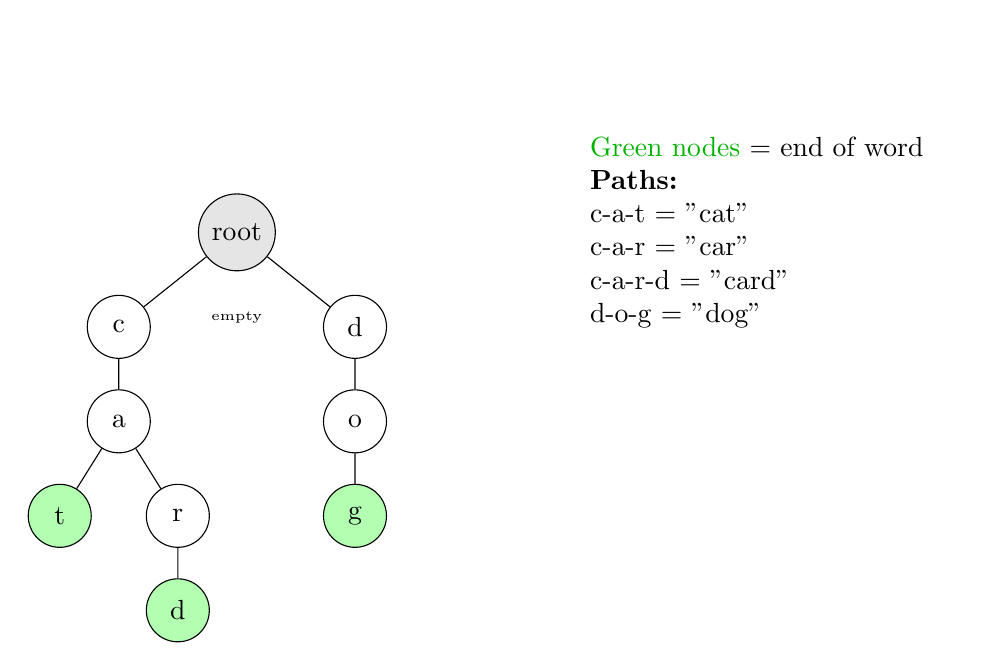
\begin{tikzpicture}[
      level distance=1.2cm,
      level 1/.style={sibling distance=3cm},
      level 2/.style={sibling distance=2cm},
      level 3/.style={sibling distance=1.5cm},
      level 4/.style={sibling distance=1cm},
      every node/.style={circle, draw, minimum size=0.8cm}
    ]
      \node[fill=gray!20] (root) {root}
        child {node {c}
          child {node {a}
            child {node[fill=green!30] {t}}
            child {node {r}
              child {node[fill=green!30] {d}}
            }
          }
        }
        child {node {d}
          child {node {o}
            child {node[fill=green!30] {g}}
          }
        };

      \node[below=0.1cm of root, draw=none] {\tiny empty};
      \node[right=3.5cm of root, draw=none, align=left] {
        \textcolor{green!70!black}{Green nodes} = end of word\\
        \textbf{Paths:}\\
        c-a-t = "cat"\\
        c-a-r = "car"\\
        c-a-r-d = "card"\\
        d-o-g = "dog"
      };
    \end{tikzpicture}
  \end{center}
\end{frame}

\begin{frame}{Why Use Tries?}
  \textbf{Advantages:}
  \begin{itemize}
    \item \textbf{Fast prefix queries:} O(m) where m = prefix length
    \item \textbf{Shared prefixes:} Memory efficient for common prefixes
    \item \textbf{Predictable performance:} No hash collisions
    \item \textbf{Alphabetical ordering:} Natural lexicographic order
  \end{itemize}

  \vspace{0.3cm}
  \textbf{Comparison with Hash Table:}
  \begin{table}
    \centering
    \small
    \begin{tabular}{|l|c|c|}
      \hline
      \textbf{Operation} & \textbf{Hash Table} & \textbf{Trie} \\
      \hline
      Search & O(1) avg & O(m) \\
      \hline
      Insert & O(1) avg & O(m) \\
      \hline
      Prefix search & O(n) & O(m + k) \\
      \hline
      Ordered traversal & O(n log n) & O(n) \\
      \hline
      Space & O(n) & O(ALPHABET * n * m) \\
      \hline
    \end{tabular}
  \end{table}

  \vspace{0.2cm}
  \small m = word length, k = results, n = number of words
\end{frame}

\begin{frame}{Common Applications}
  \textbf{Real-World Uses:}
  \begin{itemize}
    \item \textbf{Autocomplete:} Search engines, text editors
    \item \textbf{Spell checking:} Word suggestions and corrections
    \item \textbf{IP routing:} Longest prefix matching in routers
    \item \textbf{Dictionary:} Fast word lookup and validation
    \item \textbf{Phone directory:} T9 predictive text
    \item \textbf{DNA sequencing:} Pattern matching in genomics
  \end{itemize}
\end{frame}

\section{Node Structure and Implementation}

\begin{frame}[fragile]{Basic Trie Node Structure}
  \begin{lstlisting}[language=Python, basicstyle=\ttfamily\small]
class TrieNode:
    def __init__(self):
        self.children = {}  # Map: char -> TrieNode
        self.is_end_of_word = False

class Trie:
    def __init__(self):
        self.root = TrieNode()
  \end{lstlisting}

  \vspace{0.3cm}
  \textbf{Node Components:}
  \begin{itemize}
    \item \texttt{children}: Dictionary mapping characters to child nodes
    \item \texttt{is\_end\_of\_word}: Boolean flag marking complete words
  \end{itemize}

  \vspace{0.3cm}
  \textbf{Space per node:} $\sim$100+ bytes (dict overhead + bool)
\end{frame}

\begin{frame}[fragile]{Array-Based Implementation}
  \textbf{For fixed alphabets (e.g., lowercase a-z):}

  \begin{lstlisting}[language=Python, basicstyle=\ttfamily\small]
class TrieNodeArray:
    def __init__(self):
        self.children = [None] * 26  # For lowercase a-z
        self.is_end_of_word = False

    def get_index(self, char):
        return ord(char) - ord('a')

    def get_child(self, char):
        index = self.get_index(char)
        return self.children[index]

    def set_child(self, char, node):
        index = self.get_index(char)
        self.children[index] = node
  \end{lstlisting}

  \vspace{0.3cm}
  \textbf{Trade-offs:}
  \begin{itemize}
    \item \textbf{Pro:} Faster access O(1), less memory overhead per node
    \item \textbf{Con:} Wastes space if sparse (26 pointers even if only 1-2 used)
  \end{itemize}
\end{frame}

\begin{frame}[fragile]{Node with Parent Pointers}
  \textbf{Enhanced structure for traversal:}

  \begin{lstlisting}[language=Python, basicstyle=\ttfamily\small]
class TrieNodeWithParent:
    def __init__(self, char='', parent=None):
        self.char = char
        self.parent = parent
        self.children = {}
        self.is_end_of_word = False

    def get_word(self):
        """Reconstruct word from this node"""
        word = []
        node = self
        while node.parent is not None:
            word.append(node.char)
            node = node.parent
        return ''.join(reversed(word))
  \end{lstlisting}

  \vspace{0.3cm}
  \textbf{Use cases:}
  \begin{itemize}
    \item Word reconstruction without storing full strings
    \item Backtracking during searches
    \item Debugging and visualization
  \end{itemize}
\end{frame}

\section{Core Operations}

\begin{frame}[fragile]{Insert Operation}
  \begin{lstlisting}[language=Python, basicstyle=\ttfamily\small]
def insert(self, word):
    """Insert word into trie - O(m) where m = word length"""
    node = self.root

    for char in word:
        if char not in node.children:
            node.children[char] = TrieNode()
        node = node.children[char]

    node.is_end_of_word = True
  \end{lstlisting}

  \vspace{0.3cm}
  \textbf{Algorithm:}
  \begin{enumerate}
    \item Start at root
    \item For each character in word:
      \begin{itemize}
        \item If child exists, move to it
        \item Otherwise, create new child node
      \end{itemize}
    \item Mark final node as end of word
  \end{enumerate}

  \textbf{Time Complexity:} O(m) where m = length of word

  \textbf{Space Complexity:} O(m) worst case (all new nodes)
\end{frame}

\begin{frame}{Insert Visualization}
  \textbf{Inserting "car" into trie with "cat":}

  \vspace{0.3cm}
  \begin{columns}[T]
    \begin{column}{0.45\textwidth}
      \textbf{Before:}
      \begin{center}
        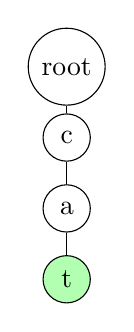
\begin{tikzpicture}[
          level distance=1cm,
          level 1/.style={sibling distance=1.5cm},
          every node/.style={circle, draw, minimum size=0.6cm},
          scale=0.9
        ]
          \node (r1) {root}
            child {node {c}
              child {node {a}
                child {node[fill=green!30] {t}}
              }
            };
        \end{tikzpicture}
      \end{center}

      Only "cat" exists
    \end{column}

    \begin{column}{0.45\textwidth}
      \textbf{After insert("car"):}
      \begin{center}
        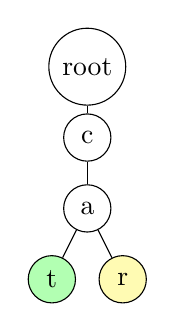
\begin{tikzpicture}[
          level distance=1cm,
          level 1/.style={sibling distance=1.5cm},
          level 2/.style={sibling distance=1cm},
          every node/.style={circle, draw, minimum size=0.6cm},
          scale=0.9
        ]
          \node (r2) {root}
            child {node {c}
              child {node {a}
                child {node[fill=green!30] {t}}
                child {node[fill=yellow!30] {r}}
              }
            };
        \end{tikzpicture}
      \end{center}

      Both "cat" and "car" exist
    \end{column}
  \end{columns}

  \vspace{0.3cm}
  \textbf{Key insight:} Common prefix "ca" is shared between words
\end{frame}

\begin{frame}[fragile]{Search Operation}
  \begin{lstlisting}[language=Python, basicstyle=\ttfamily\small]
def search(self, word):
    """Search for exact word - O(m)"""
    node = self.root

    for char in word:
        if char not in node.children:
            return False
        node = node.children[char]

    return node.is_end_of_word
  \end{lstlisting}

  \vspace{0.3cm}
  \textbf{Examples:}
  \begin{itemize}
    \item \texttt{search("cat")} $\rightarrow$ \textcolor{green}{True} (complete word)
    \item \texttt{search("ca")} $\rightarrow$ \textcolor{red}{False} (prefix but not word)
    \item \texttt{search("cats")} $\rightarrow$ \textcolor{red}{False} (doesn't exist)
  \end{itemize}

  \vspace{0.3cm}
  \textbf{Important:} Must check \texttt{is\_end\_of\_word} flag!

  Just reaching a node doesn't mean the word exists.
\end{frame}

\begin{frame}[fragile]{Prefix Search (Starts With)}
  \begin{lstlisting}[language=Python, basicstyle=\ttfamily\small]
def starts_with(self, prefix):
    """Check if any word starts with prefix - O(m)"""
    node = self.root

    for char in prefix:
        if char not in node.children:
            return False
        node = node.children[char]

    return True  # No need to check is_end_of_word
  \end{lstlisting}

  \vspace{0.3cm}
  \textbf{Difference from search:}
  \begin{itemize}
    \item Don't check \texttt{is\_end\_of\_word}
    \item Just verify path exists
  \end{itemize}

  \vspace{0.3cm}
  \textbf{Examples with trie containing ["cat", "car", "card"]:}
  \begin{itemize}
    \item \texttt{starts\_with("ca")} $\rightarrow$ \textcolor{green}{True}
    \item \texttt{starts\_with("car")} $\rightarrow$ \textcolor{green}{True}
    \item \texttt{starts\_with("dog")} $\rightarrow$ \textcolor{red}{False}
  \end{itemize}
\end{frame}

\begin{frame}[fragile]{Delete Operation}
  \begin{lstlisting}[language=Python, basicstyle=\ttfamily\footnotesize]
def delete(self, word):
    """Delete word from trie - O(m)"""
    def _delete(node, word, index):
        if index == len(word):
            # Reached end of word
            if not node.is_end_of_word:
                return False  # Word doesn't exist

            node.is_end_of_word = False

            # Return True if node has no children (can be deleted)
            return len(node.children) == 0

        char = word[index]
        if char not in node.children:
            return False  # Word doesn't exist

        child = node.children[char]
        should_delete_child = _delete(child, word, index + 1)

        if should_delete_child:
            del node.children[char]
            # Return True if current node can be deleted
            return len(node.children) == 0 and not node.is_end_of_word

        return False

    _delete(self.root, word, 0)
  \end{lstlisting}
\end{frame}

\begin{frame}{Delete Visualization}
  \textbf{Deleting "car" from trie with ["cat", "car", "card"]:}

  \vspace{0.3cm}
  \begin{columns}[T]
    \begin{column}{0.45\textwidth}
      \textbf{Before delete("car"):}
      \begin{center}
        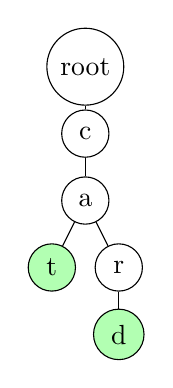
\begin{tikzpicture}[
          level distance=1cm,
          level 1/.style={sibling distance=1.5cm},
          level 2/.style={sibling distance=1cm},
          every node/.style={circle, draw, minimum size=0.6cm},
          scale=0.85
        ]
          \node {root}
            child {node {c}
              child {node {a}
                child {node[fill=green!30] {t}}
                child {node {r}
                  child {node[fill=green!30] {d}}
                }
              }
            };
        \end{tikzpicture}
      \end{center}
    \end{column}

    \begin{column}{0.45\textwidth}
      \textbf{After delete("car"):}
      \begin{center}
        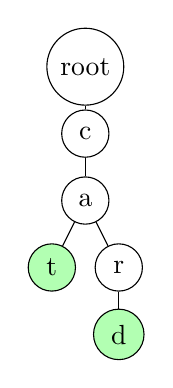
\begin{tikzpicture}[
          level distance=1cm,
          level 1/.style={sibling distance=1.5cm},
          level 2/.style={sibling distance=1cm},
          every node/.style={circle, draw, minimum size=0.6cm},
          scale=0.85
        ]
          \node {root}
            child {node {c}
              child {node {a}
                child {node[fill=green!30] {t}}
                child {node {r}
                  child {node[fill=green!30] {d}}
                }
              }
            };
        \end{tikzpicture}
      \end{center}
    \end{column}
  \end{columns}

  \vspace{0.3cm}
  \textbf{Key points:}
  \begin{itemize}
    \item Node 'r' is NOT deleted (needed by "card")
    \item Only the \texttt{is\_end\_of\_word} flag on 'r' is set to false
    \item Nodes deleted only if they have no children and aren't word endings
  \end{itemize}
\end{frame}

\section{Prefix Queries and Autocomplete}

\begin{frame}[fragile]{Find All Words with Prefix}
  \begin{lstlisting}[language=Python, basicstyle=\ttfamily\footnotesize]
def find_words_with_prefix(self, prefix):
    """Return all words starting with prefix"""
    node = self.root

    # Navigate to prefix node
    for char in prefix:
        if char not in node.children:
            return []
        node = node.children[char]

    # Collect all words from this node
    words = []
    self._collect_words(node, prefix, words)
    return words

def _collect_words(self, node, current_word, words):
    """DFS to collect all words from node"""
    if node.is_end_of_word:
        words.append(current_word)

    for char, child in node.children.items():
        self._collect_words(child, current_word + char, words)
  \end{lstlisting}

  \textbf{Time Complexity:} O(p + n) where p = prefix length, n = matching words
\end{frame}

\begin{frame}{Prefix Query Example}
  \textbf{Trie with words:} ["cat", "car", "card", "care", "dog"]

  \vspace{0.3cm}
  \begin{center}
    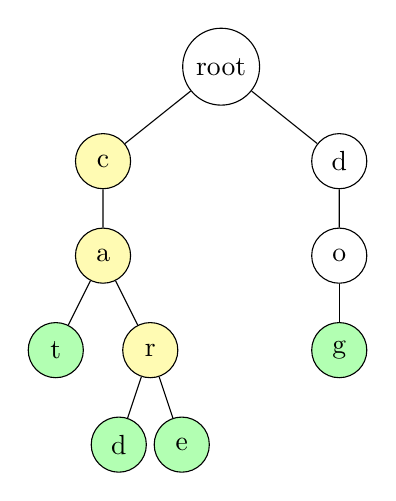
\begin{tikzpicture}[
      level distance=1.2cm,
      level 1/.style={sibling distance=3cm},
      level 2/.style={sibling distance=2cm},
      level 3/.style={sibling distance=1.2cm},
      level 4/.style={sibling distance=0.8cm},
      every node/.style={circle, draw, minimum size=0.7cm}
    ]
      \node {root}
        child {node[fill=yellow!30] {c}
          child {node[fill=yellow!30] {a}
            child {node[fill=green!30] {t}}
            child {node[fill=yellow!30] {r}
              child {node[fill=green!30] {d}}
              child {node[fill=green!30] {e}}
            }
          }
        }
        child {node {d}
          child {node {o}
            child {node[fill=green!30] {g}}
          }
        };
    \end{tikzpicture}
  \end{center}

  \vspace{0.3cm}
  \texttt{find\_words\_with\_prefix("car")} $\rightarrow$ ["car", "card", "care"]

  \textcolor{yellow!70!black}{Yellow} shows path to prefix, then DFS collects \textcolor{green!70!black}{green} endings
\end{frame}

\begin{frame}[fragile]{Autocomplete with Limit}
  \begin{lstlisting}[language=Python, basicstyle=\ttfamily\footnotesize]
def autocomplete(self, prefix, max_results=5):
    """Return top N autocomplete suggestions"""
    node = self.root

    # Navigate to prefix
    for char in prefix:
        if char not in node.children:
            return []
        node = node.children[char]

    # BFS to find closest words
    from collections import deque
    results = []
    queue = deque([(node, prefix)])

    while queue and len(results) < max_results:
        current, word = queue.popleft()

        if current.is_end_of_word:
            results.append(word)

        for char, child in sorted(current.children.items()):
            queue.append((child, word + char))

    return results
  \end{lstlisting}
\end{frame}

\begin{frame}[fragile]{Longest Common Prefix}
  \begin{lstlisting}[language=Python, basicstyle=\ttfamily\small]
def longest_common_prefix(self, words):
    """Find longest common prefix of all words"""
    if not words:
        return ""

    # Insert all words
    for word in words:
        self.insert(word)

    # Traverse until branching or end
    node = self.root
    prefix = ""

    while len(node.children) == 1 and not node.is_end_of_word:
        char = next(iter(node.children))
        prefix += char
        node = node.children[char]

    return prefix
  \end{lstlisting}

  \vspace{0.3cm}
  \textbf{Example:}
  \begin{itemize}
    \item Input: ["flower", "flow", "flight"]
    \item Output: "fl"
  \end{itemize}
\end{frame}

\begin{frame}[fragile]{Wildcard Search}
  \begin{lstlisting}[language=Python, basicstyle=\ttfamily\footnotesize]
def search_with_wildcard(self, pattern):
    """Search with '.' as wildcard for any character"""
    def dfs(node, index):
        if index == len(pattern):
            return node.is_end_of_word

        char = pattern[index]

        if char == '.':
            # Try all children
            for child in node.children.values():
                if dfs(child, index + 1):
                    return True
            return False
        else:
            if char not in node.children:
                return False
            return dfs(node.children[char], index + 1)

    return dfs(self.root, 0)
  \end{lstlisting}

  \vspace{0.3cm}
  \textbf{Examples:}
  \begin{itemize}
    \item \texttt{search\_with\_wildcard("c.r")} matches "car"
    \item \texttt{search\_with\_wildcard("c..")} matches "cat", "car"
  \end{itemize}
\end{frame}

\section{Memory Optimization}

\begin{frame}{Memory Usage Analysis}
  \textbf{Standard Trie Space Complexity:}

  \vspace{0.3cm}
  For words ["cat", "car", "card"]:
  \begin{itemize}
    \item Nodes: root + c + a + t + r + d = 6 nodes
    \item Each node: dict (hash table) + bool $\approx$ 100+ bytes
    \item Total: $\sim$600 bytes for 3 words
  \end{itemize}

  \vspace{0.3cm}
  \textbf{Worst Case: No shared prefixes}

  Words: ["abc", "def", "ghi"]
  \begin{itemize}
    \item Nodes: 1 + 3*3 = 10 nodes
    \item Space: O(ALPHABET\_SIZE $\times$ N $\times$ M)
    \item N = number of words, M = average length
  \end{itemize}

  \vspace{0.3cm}
  \textbf{Best Case: Many shared prefixes}

  Words: ["test", "testing", "tester"]
  \begin{itemize}
    \item Much better space efficiency due to sharing
  \end{itemize}
\end{frame}

\begin{frame}{Radix Tree (Compressed Trie)}
  \textbf{Idea:} Merge chains of single-child nodes

  \vspace{0.3cm}
  \begin{columns}[T]
    \begin{column}{0.45\textwidth}
      \textbf{Standard Trie:}
      \begin{center}
        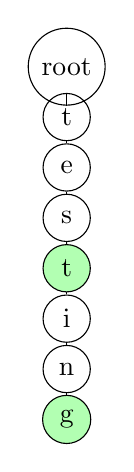
\begin{tikzpicture}[
          level distance=0.8cm,
          every node/.style={circle, draw, minimum size=0.6cm},
          scale=0.8
        ]
          \node {root}
            child {node {t}
              child {node {e}
                child {node {s}
                  child {node[fill=green!30] {t}
                    child {node {i}
                      child {node {n}
                        child {node[fill=green!30] {g}}
                      }
                    }
                  }
                }
              }
            };
        \end{tikzpicture}
      \end{center}
      9 nodes
    \end{column}

    \begin{column}{0.45\textwidth}
      \textbf{Radix Tree:}
      \begin{center}
        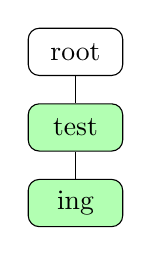
\begin{tikzpicture}[
          level distance=1.2cm,
          every node/.style={rectangle, draw, rounded corners, minimum width=1.2cm, minimum height=0.6cm},
          scale=0.8
        ]
          \node {root}
            child {node[fill=green!30] {test}
              child {node[fill=green!30] {ing}}
            };
        \end{tikzpicture}
      \end{center}
      3 nodes (67\% reduction)
    \end{column}
  \end{columns}

  \vspace{0.3cm}
  \textbf{Trade-offs:}
  \begin{itemize}
    \item \textbf{Pro:} O(N) nodes where N = number of words
    \item \textbf{Con:} More complex implementation (node splitting)
  \end{itemize}
\end{frame}

\begin{frame}[fragile]{Radix Node Structure}
  \begin{lstlisting}[language=Python, basicstyle=\ttfamily\small]
class RadixNode:
    def __init__(self, label=""):
        self.label = label  # String, not single char!
        self.children = {}
        self.is_end_of_word = False

class RadixTree:
    def __init__(self):
        self.root = RadixNode()
  \end{lstlisting}

  \vspace{0.3cm}
  \textbf{Key Difference:}
  \begin{itemize}
    \item Standard Trie: Each node stores one character
    \item Radix Tree: Each node stores a string (edge label)
  \end{itemize}

  \vspace{0.3cm}
  \textbf{Applications:}
  \begin{itemize}
    \item Git uses radix trees internally
    \item Linux kernel routing tables
    \item Memory-efficient string storage
  \end{itemize}
\end{frame}

\begin{frame}{Space Optimization Techniques}
  \textbf{1. Array-based for small alphabets}
  \begin{itemize}
    \item Use fixed-size array instead of dictionary
    \item Trade: wastes space if sparse, but faster access
  \end{itemize}

  \vspace{0.3cm}
  \textbf{2. Bit packing for flags}
  \begin{itemize}
    \item Pack multiple boolean flags into single integer
    \item Saves memory when nodes have many flags
  \end{itemize}

  \vspace{0.3cm}
  \textbf{3. Lazy initialization}
  \begin{itemize}
    \item Don't create children dict until needed
    \item \texttt{self.children = None} initially
  \end{itemize}

  \vspace{0.3cm}
  \textbf{4. Use radix tree for long common prefixes}
  \begin{itemize}
    \item Significantly reduces node count
    \item Best for datasets with long shared prefixes
  \end{itemize}
\end{frame}

\section{Enhanced Tries with Metadata}

\begin{frame}[fragile]{Frequency Trie}
  \textbf{Store word frequencies for autocomplete ranking:}

  \begin{lstlisting}[language=Python, basicstyle=\ttfamily\small]
class FrequencyTrieNode:
    def __init__(self):
        self.children = {}
        self.count = 0  # Number of times word inserted

class FrequencyTrie:
    def __init__(self):
        self.root = FrequencyTrieNode()

    def insert(self, word):
        node = self.root
        for char in word:
            if char not in node.children:
                node.children[char] = FrequencyTrieNode()
            node = node.children[char]
        node.count += 1

    def get_frequency(self, word):
        node = self.root
        for char in word:
            if char not in node.children:
                return 0
            node = node.children[char]
        return node.count
  \end{lstlisting}
\end{frame}

\begin{frame}[fragile]{Top-K Autocomplete with Frequency}
  \begin{lstlisting}[language=Python, basicstyle=\ttfamily\footnotesize]
def top_k_with_prefix(self, prefix, k):
    """Get top k most frequent words with prefix"""
    node = self.root

    # Navigate to prefix
    for char in prefix:
        if char not in node.children:
            return []
        node = node.children[char]

    # Collect all words with frequencies
    words = []
    self._collect_with_freq(node, prefix, words)

    # Sort by frequency and return top k
    words.sort(key=lambda x: x[1], reverse=True)
    return [word for word, freq in words[:k]]

def _collect_with_freq(self, node, word, words):
    if node.count > 0:
        words.append((word, node.count))

    for char, child in node.children.items():
        self._collect_with_freq(child, word + char, words)
  \end{lstlisting}
\end{frame}

\begin{frame}[fragile]{Indexed Trie for Search Engines}
  \begin{lstlisting}[language=Python, basicstyle=\ttfamily\footnotesize]
class IndexedTrieNode:
    def __init__(self):
        self.children = {}
        self.doc_ids = []  # List of document IDs

class SearchEngine:
    def __init__(self):
        self.trie = IndexedTrieNode()
        self.documents = {}

    def add_document(self, doc_id, text):
        """Index document for search"""
        self.documents[doc_id] = text
        words = text.lower().split()

        for word in words:
            node = self.trie
            for char in word:
                if char not in node.children:
                    node.children[char] = IndexedTrieNode()
                node = node.children[char]

            if doc_id not in node.doc_ids:
                node.doc_ids.append(doc_id)
  \end{lstlisting}
\end{frame}

\begin{frame}[fragile]{Suffix Trie for Pattern Matching}
  \begin{lstlisting}[language=Python, basicstyle=\ttfamily\footnotesize]
class SuffixTrie:
    """Store all suffixes of a string for fast pattern matching"""
    def __init__(self, text):
        self.root = TrieNode()
        self.text = text

        # Insert all suffixes
        for i in range(len(text)):
            self._insert_suffix(text[i:], i)

    def _insert_suffix(self, suffix, start_index):
        node = self.root
        for char in suffix:
            if char not in node.children:
                node.children[char] = TrieNode()
            node = node.children[char]
        node.start_index = start_index

    def find_pattern(self, pattern):
        """Find all occurrences of pattern in O(m + k)"""
        node = self.root
        for char in pattern:
            if char not in node.children:
                return []
            node = node.children[char]

        # Collect all start indices
        indices = []
        self._collect_indices(node, indices)
        return indices
  \end{lstlisting}
\end{frame}

\section{Real-World Applications}

\begin{frame}[fragile]{Spell Checker}
  \begin{lstlisting}[language=Python, basicstyle=\ttfamily\footnotesize]
class SpellChecker:
    def __init__(self, dictionary):
        self.trie = Trie()
        for word in dictionary:
            self.trie.insert(word.lower())

    def is_correct(self, word):
        """Check if word is spelled correctly"""
        return self.trie.search(word.lower())

    def suggest_corrections(self, word, max_distance=2):
        """Suggest corrections using edit distance"""
        suggestions = []

        def dfs(node, current, remaining_edits):
            if remaining_edits < 0:
                return

            if node.is_end_of_word and current:
                suggestions.append(current)

            # Try all possible edits...
            # (substitution, insertion, deletion)

        dfs(self.trie.root, "", max_distance)
        return suggestions[:5]
  \end{lstlisting}
\end{frame}

\begin{frame}{Spell Checker Example}
  \textbf{Dictionary:} ["cat", "car", "card", "care", "careful"]

  \vspace{0.3cm}
  \textbf{Operations:}
  \begin{itemize}
    \item \texttt{is\_correct("car")} $\rightarrow$ \textcolor{green}{True}
    \item \texttt{is\_correct("cra")} $\rightarrow$ \textcolor{red}{False}
    \item \texttt{suggest\_corrections("cra")} $\rightarrow$ ["car", "care", "card"]
  \end{itemize}

  \vspace{0.3cm}
  \textbf{Edit Distance Techniques:}
  \begin{itemize}
    \item \textbf{Substitution:} "cra" $\rightarrow$ "car" (distance = 1)
    \item \textbf{Insertion:} "cra" $\rightarrow$ "care" (distance = 1)
    \item \textbf{Deletion:} "crat" $\rightarrow$ "cat" (distance = 1)
  \end{itemize}

  \vspace{0.3cm}
  \textbf{Complexity:} O(m $\times$ ALPHABET\_SIZE$^d$) where d = max distance
\end{frame}

\begin{frame}[fragile]{IP Routing Table}
  \begin{lstlisting}[language=Python, basicstyle=\ttfamily\footnotesize]
class IPRoutingTable:
    """Longest prefix matching for IP routing"""
    def __init__(self):
        self.root = TrieNode()

    def add_route(self, ip_prefix, next_hop):
        """Add routing entry (e.g., "192.168.0.0/16")"""
        binary = self._ip_to_binary(ip_prefix)

        node = self.root
        for bit in binary:
            if bit not in node.children:
                node.children[bit] = TrieNode()
            node = node.children[bit]

        node.next_hop = next_hop
        node.is_end_of_word = True

    def lookup(self, ip_address):
        """Find longest matching prefix"""
        binary = self._ip_to_binary(ip_address)
        node = self.root
        last_match = None

        for bit in binary:
            if bit not in node.children:
                break
            node = node.children[bit]
            if node.is_end_of_word:
                last_match = node.next_hop

        return last_match
  \end{lstlisting}
\end{frame}

\begin{frame}{IP Routing Example}
  \textbf{Routing table entries:}
  \begin{itemize}
    \item 192.168.0.0/16 $\rightarrow$ Router A
    \item 192.168.1.0/24 $\rightarrow$ Router B
    \item 192.168.1.128/25 $\rightarrow$ Router C
  \end{itemize}

  \vspace{0.3cm}
  \textbf{Lookups (longest prefix match):}
  \begin{itemize}
    \item 192.168.1.200 $\rightarrow$ Router B (/24 match)
    \item 192.168.1.150 $\rightarrow$ Router C (/25 match, longest!)
    \item 192.168.2.1 $\rightarrow$ Router A (/16 match)
  \end{itemize}

  \vspace{0.3cm}
  \textbf{Why Trie?}
  \begin{itemize}
    \item Fast O(32) lookup for IPv4 (32 bits)
    \item Naturally finds longest prefix
    \item Efficient for large routing tables
  \end{itemize}
\end{frame}

\begin{frame}[fragile]{Autocomplete System}
  \begin{lstlisting}[language=Python, basicstyle=\ttfamily\footnotesize]
class AutocompleteSystem:
    """Google-style autocomplete with frequency ranking"""
    def __init__(self):
        self.trie = FrequencyTrie()
        self.current_prefix = ""

    def input(self, char):
        """Process one character input"""
        if char == '#':
            # End of sentence, save it
            self.trie.insert(self.current_prefix)
            self.current_prefix = ""
            return []

        self.current_prefix += char

        # Return top 3 suggestions
        return self.trie.top_k_with_prefix(self.current_prefix, 3)
  \end{lstlisting}

  \vspace{0.3cm}
  \textbf{Usage:}
  \begin{itemize}
    \item User types 'c' $\rightarrow$ Show ["cat", "car", "card"]
    \item User types 'a' $\rightarrow$ Show ["cat", "car", "card"]
    \item User types 'r' $\rightarrow$ Show ["car", "card", "care"]
    \item User types '\#' $\rightarrow$ Save "car", increment frequency
  \end{itemize}
\end{frame}

\begin{frame}[fragile]{Word Break Problem}
  \begin{lstlisting}[language=Python, basicstyle=\ttfamily\footnotesize]
def word_break(s, word_dict):
    """Check if string can be segmented into dictionary words
    Example: "leetcode" with ["leet", "code"] -> True
    """
    trie = Trie()
    for word in word_dict:
        trie.insert(word)

    n = len(s)
    dp = [False] * (n + 1)
    dp[0] = True  # Empty string

    for i in range(1, n + 1):
        node = trie.root
        for j in range(i - 1, -1, -1):
            if not dp[j]:
                continue

            char = s[j]
            if char not in node.children:
                break

            node = node.children[char]

            if node.is_end_of_word:
                dp[i] = True
                break

    return dp[n]
  \end{lstlisting}
\end{frame}

\begin{frame}[fragile]{File System Path Matching}
  \begin{lstlisting}[language=Python, basicstyle=\ttfamily\footnotesize]
class FileSystemTrie:
    """Efficient file path matching with wildcards"""
    def __init__(self):
        self.root = TrieNode()

    def add_path(self, path):
        """Add file path like /home/user/file.txt"""
        parts = path.strip('/').split('/')
        node = self.root

        for part in parts:
            if part not in node.children:
                node.children[part] = TrieNode()
            node = node.children[part]

        node.is_end_of_word = True

    def find_files(self, pattern):
        """Find files matching pattern (e.g., /home/*/file.txt)"""
        parts = pattern.strip('/').split('/')
        results = []

        def dfs(node, index, current_path):
            if index == len(parts):
                if node.is_end_of_word:
                    results.append(current_path)
                return

            if parts[index] == '*':
                # Wildcard matches any directory
                for name, child in node.children.items():
                    dfs(child, index + 1, current_path + '/' + name)
            else:
                if parts[index] in node.children:
                    dfs(node.children[parts[index]], index + 1,
                        current_path + '/' + parts[index])

        dfs(self.root, 0, "")
        return results
  \end{lstlisting}
\end{frame}

\section{Complexity Analysis}

\begin{frame}{Time Complexity Summary}
  \begin{table}
    \centering
    \begin{tabular}{|l|c|c|}
      \hline
      \textbf{Operation} & \textbf{Time Complexity} & \textbf{Notes} \\
      \hline
      Insert & O(m) & m = word length \\
      \hline
      Search & O(m) & Exact word search \\
      \hline
      Delete & O(m) & Recursive cleanup \\
      \hline
      Prefix search & O(p) & p = prefix length \\
      \hline
      Find all with prefix & O(p + n) & n = matching words \\
      \hline
      Autocomplete (top k) & O(p + k) & k = results returned \\
      \hline
      Wildcard search & O(m $\times$ b$^w$) & w = wildcards, b = branching \\
      \hline
    \end{tabular}
  \end{table}

  \vspace{0.5cm}
  \textbf{Key Insight:} Performance depends on word/prefix length, NOT total words!

  This makes tries excellent for large dictionaries.
\end{frame}

\begin{frame}{Space Complexity Summary}
  \textbf{Standard Trie:}
  \begin{itemize}
    \item \textbf{Best case:} O(m) where m = longest word (all words share prefix)
    \item \textbf{Average case:} O(ALPHABET\_SIZE $\times$ n $\times$ m)
    \item \textbf{Worst case:} O(ALPHABET\_SIZE $\times$ n $\times$ m) (no shared prefixes)
  \end{itemize}

  \vspace{0.3cm}
  \textbf{Radix Tree:}
  \begin{itemize}
    \item O(n) nodes where n = number of words
    \item Much better space efficiency
  \end{itemize}

  \vspace{0.3cm}
  \textbf{Space Optimization Trade-offs:}
  \begin{table}
    \centering
    \small
    \begin{tabular}{|l|c|c|}
      \hline
      \textbf{Implementation} & \textbf{Space} & \textbf{Speed} \\
      \hline
      Dictionary-based & High & Fast \\
      \hline
      Array-based (sparse) & Very High & Fastest \\
      \hline
      Array-based (dense) & Medium & Fastest \\
      \hline
      Radix tree & Low & Medium \\
      \hline
    \end{tabular}
  \end{table}
\end{frame}

\begin{frame}{Comparison with Other Data Structures}
  \begin{table}
    \centering
    \small
    \begin{tabular}{|l|c|c|c|}
      \hline
      \textbf{Feature} & \textbf{Hash Table} & \textbf{BST} & \textbf{Trie} \\
      \hline
      Insert & O(1) & O(log n) & O(m) \\
      \hline
      Search & O(1) & O(log n) & O(m) \\
      \hline
      Delete & O(1) & O(log n) & O(m) \\
      \hline
      Prefix search & O(n) & O(n) & O(p + k) \\
      \hline
      Sorted order & No & Yes & Yes \\
      \hline
      Space & O(n) & O(n) & O(n $\times$ m) \\
      \hline
      Collisions & Yes & No & No \\
      \hline
    \end{tabular}
  \end{table}

  \vspace{0.3cm}
  \textbf{When to use Trie:}
  \begin{itemize}
    \item Need prefix-based queries (autocomplete, spell check)
    \item Many words with common prefixes
    \item Need predictable performance (no hash collisions)
    \item Lexicographic ordering matters
  \end{itemize}
\end{frame}

\section{Summary}

\begin{frame}{Key Concepts Recap}
  \textbf{Trie Fundamentals:}
  \begin{itemize}
    \item Tree where each node = character
    \item Path from root = string/prefix
    \item Efficient prefix queries: O(m) not O(n)
  \end{itemize}

  \vspace{0.3cm}
  \textbf{Core Operations:}
  \begin{itemize}
    \item Insert, Search, Delete: All O(m)
    \item Prefix search: O(p)
    \item Find all with prefix: O(p + n)
  \end{itemize}

  \vspace{0.3cm}
  \textbf{Variants:}
  \begin{itemize}
    \item Dictionary-based (flexible alphabet)
    \item Array-based (fixed alphabet, faster)
    \item Radix tree (compressed, space-efficient)
    \item Frequency trie (ranking autocomplete)
  \end{itemize}
\end{frame}

\begin{frame}{Applications Recap}
  \textbf{Major Use Cases:}
  \begin{itemize}
    \item \textbf{Autocomplete:} Search engines, text editors
    \item \textbf{Spell checking:} Word processors
    \item \textbf{IP routing:} Network routers (longest prefix match)
    \item \textbf{Text search:} Pattern matching, substring search
    \item \textbf{Dictionary:} Fast word validation
    \item \textbf{DNA sequencing:} Genomic pattern matching
  \end{itemize}

  \vspace{0.3cm}
  \textbf{When NOT to use Trie:}
  \begin{itemize}
    \item Simple exact-match lookups (use hash table)
    \item No prefix queries needed
    \item Memory is very limited
    \item Small, simple datasets
  \end{itemize}
\end{frame}

\begin{frame}{Practice Problems}
  \textbf{Basic:}
  \begin{itemize}
    \item Implement insert, search, starts\_with operations
    \item Find longest common prefix of array of strings
    \item Count words with given prefix
  \end{itemize}

  \vspace{0.3cm}
  \textbf{Intermediate:}
  \begin{itemize}
    \item Implement autocomplete with top-k results
    \item Word search with wildcards
    \item Design search autocomplete system (LeetCode 642)
    \item Word break problem using trie
  \end{itemize}

  \vspace{0.3cm}
  \textbf{Advanced:}
  \begin{itemize}
    \item Implement radix tree with node splitting
    \item Design spell checker with edit distance
    \item Suffix tree construction and pattern matching
    \item Trie with frequency-based ranking
  \end{itemize}
\end{frame}

\begin{frame}{Implementation Tips}
  \textbf{Best Practices:}
  \begin{itemize}
    \item Use dictionary for variable alphabets (UTF-8, symbols)
    \item Use array for fixed alphabets (a-z, 0-9)
    \item Consider radix tree if memory is concern
    \item Add metadata (frequency, indices) for advanced features
  \end{itemize}

  \vspace{0.3cm}
  \textbf{Common Pitfalls:}
  \begin{itemize}
    \item Forgetting to check \texttt{is\_end\_of\_word} in search
    \item Not handling empty string correctly
    \item Memory leaks in delete operation
    \item Not considering case sensitivity
  \end{itemize}

  \vspace{0.3cm}
  \textbf{Optimization Strategies:}
  \begin{itemize}
    \item Cache frequently accessed nodes
    \item Use lazy initialization for children
    \item Implement iterative versions to avoid recursion overhead
    \item Profile and optimize hot paths
  \end{itemize}
\end{frame}

\begin{frame}{Further Learning}
  \textbf{Related Topics:}
  \begin{itemize}
    \item \textbf{Suffix Trees:} All suffixes of a string
    \item \textbf{Ternary Search Trees:} Space-efficient alternative
    \item \textbf{Patricia Trees:} Practical Algorithm to Retrieve Information
    \item \textbf{Aho-Corasick:} Multiple pattern matching
  \end{itemize}

  \vspace{0.3cm}
  \textbf{Resources:}
  \begin{itemize}
    \item Implement all operations from scratch
    \item LeetCode Trie problems (208, 211, 212, 642, 648)
    \item Real-world project: Build autocomplete system
    \item Study open-source implementations (Redis, Elasticsearch)
  \end{itemize}

  \vspace{0.3cm}
  \textbf{Projects:}
  \begin{itemize}
    \item Search autocomplete with frequency ranking
    \item Spell checker with suggestions
    \item T9 predictive text system
    \item Simple search engine with trie indexing
  \end{itemize}
\end{frame}

\begin{frame}
  \begin{center}
    {\Huge Thank You!}

    \vspace{1cm}
    {\Large Questions?}

    \vspace{1cm}
    \textbf{Tries: Mastering Prefix-Based Queries}
  \end{center}
\end{frame}

\end{document}
